\begin{frame}
\frametitle{Introductory Calculus--Infinitesimal Approach}
\framesubtitle{1.4 Slope And Velocity; The Hyperreal Line 02}
\label{slide:1.4-02}
\begin{itemize}
\item \begin{figure}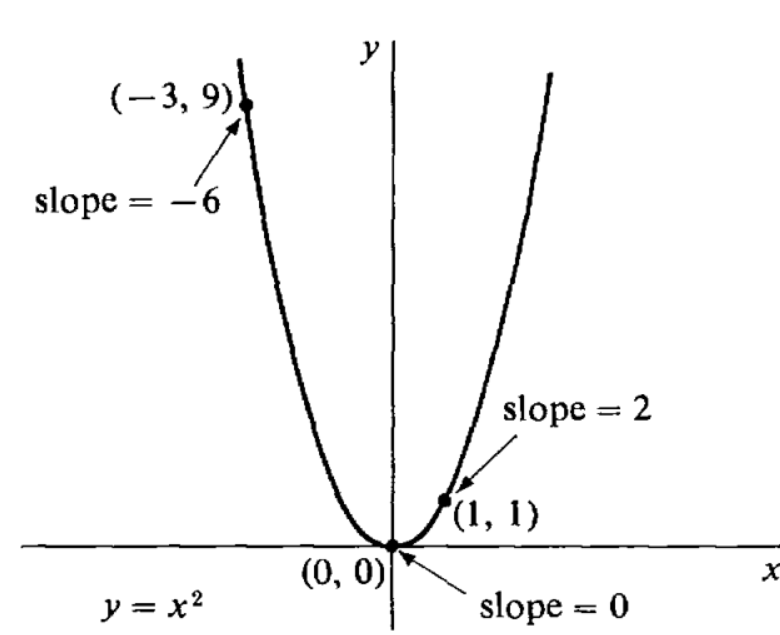
\includegraphics[width=.5\textwidth]{images/slope-examples-parabola}\end{figure}
\pause\item For Example, The Slope Is $2x_0=2\cdot 0=0$ at $(0,0)$, $2\cdot 1=2$ at $(1,1)$, And $2\cdot -3=-6$ at $(-3, 9)$.
\end{itemize}
\end{frame}
